\section{Formulation of the Mini-Golf Problem}

\begin{figure}[H]
	\centering
	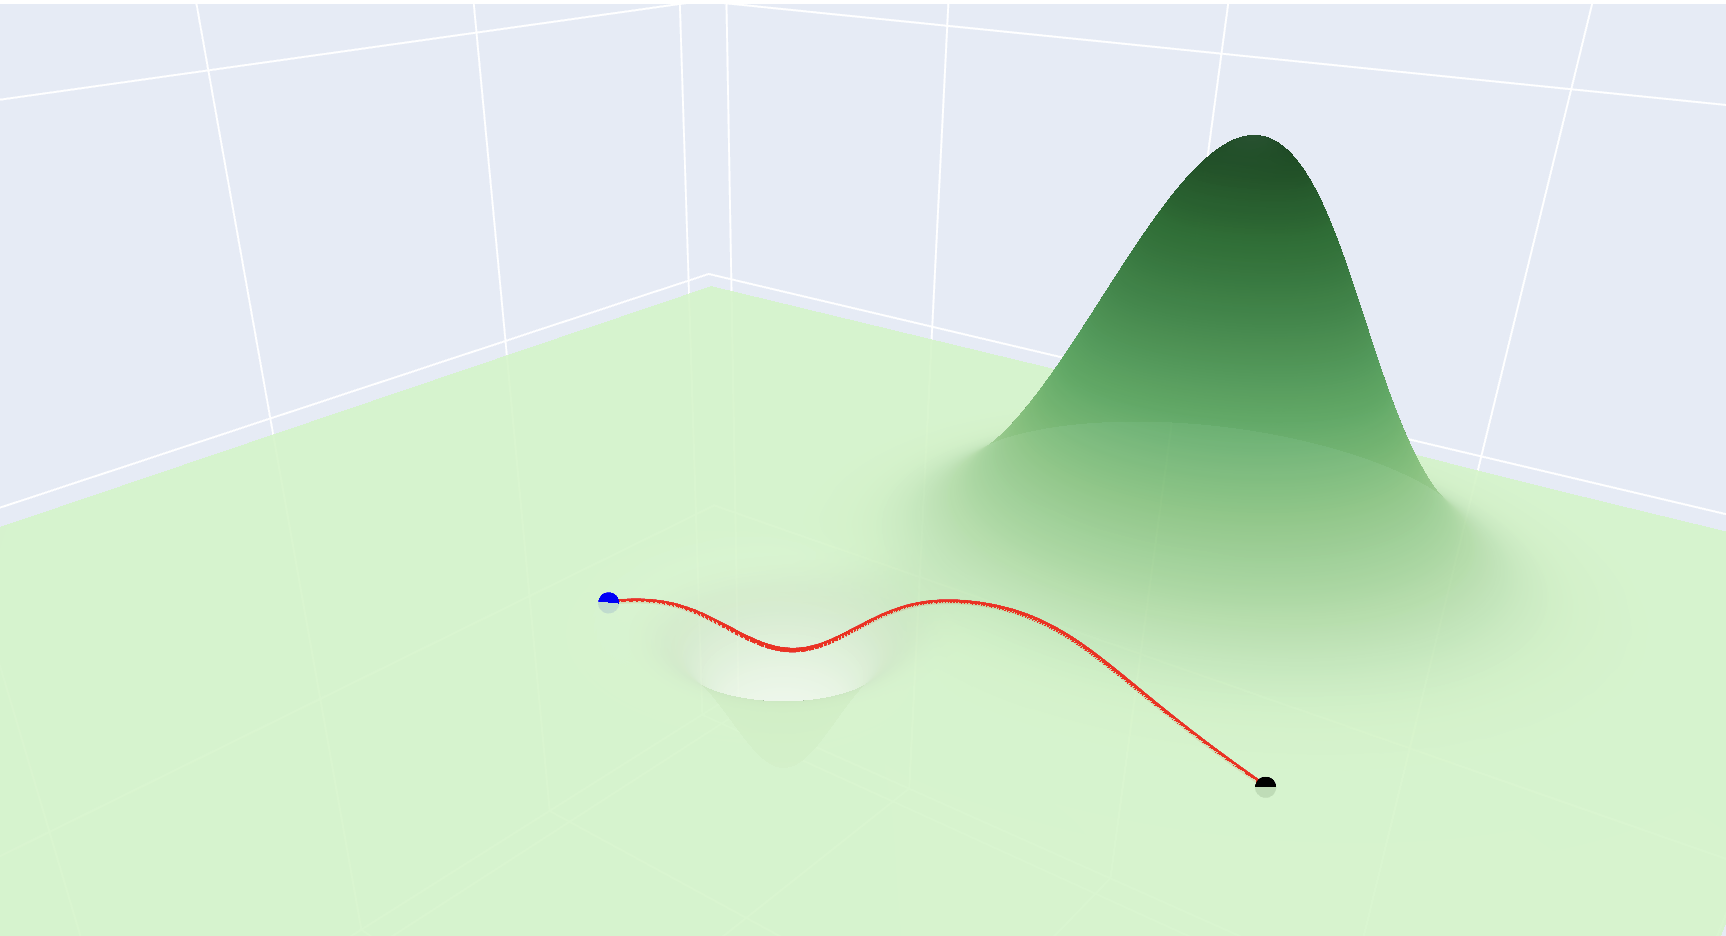
\includegraphics[width=0.75\textwidth]{assets/minigolf_pic.png}
	\caption{A simple diagram depicting the way that a golf ball moves on some golf course. The goal of this investigation is to determine the trajectory, e.g. the red line in the image, given an initial starting position $(q_1,q_2)$ and velocity $(\dot q_1, \dot q_2)$.}
	\label{fig:golf1}
	% Source: https://en.wikiversity.org/wiki/Continuum_mechanics/Calculus_of_variations
\end{figure}

Since our golf ball lives in 3 dimensions (since we are 3D creatures), we can express the golf balls' position as a 3 dimensional vector of x,y, and z coordinates, $q_1, q_2$, and $q_3$ respectively. Thus, let us denote the position vector of the golf ball as

\begin{equation}
	\vec q = \begin{pmatrix}
		q_1\\
		q_2\\
		q_3
	\end{pmatrix}= (q_1,q_2,q_3)^T.
\end{equation}

This golf ball is bound permanently to a golf course, which we will define as a twice continuously-differentiable surface $q_z=h(q_x,q_y)$. This means that all first and second-order partial derivatives of $h$, ($\partial_i h, \partial_{ij}h$, $i,j=1,2,3$) exist and are continuous. From now on, let $\partial_i h = \frac{\partial h}{\partial q_i}$ for sake of notational simplicity. Recall from \ref{holconstraint} that we directly introduced the holonomic constraint of the golf ball system as

\begin{equation}
	q_3=h(q_1,q_2),
\end{equation}

which simplifies our expression of the golf ball position to only two generalized coordinates: $q_1$ and $q_2$. Now, our originally 3D position $\vec q \in \mathbb{R}^3$ can be reduced to a 2D vector of generalized coordinates e.g.

\begin{equation}
	\vec q = \begin{pmatrix}
		q_1 \\
		q_2
	\end{pmatrix}.
\end{equation}

With our system defined, and our generalized coordinates $q_1, q_2$ linked to the physical state of the golfball on the course $h(q_1,q_2)$, let us continue to construct the Lagrangian formalism described in Section 2. Since the Lagrangian function is given as the difference between the kinetic and potential energy $T,V$, let us determine these energies of our golf ball in terms of our new generalized coordinates. From kinematics, it is well known that the kinetic energy of a mass $m$ at velocity $\dot q$ is given by

\begin{equation}
	T(\dot q) = \frac{1}{2}m\dot q^2
\end{equation}

Thus, the kinetic energy of the golf ball as it rolls across the minigolf course is:

\begin{equation}
	T_{ball}=\frac{1}{2}m\|\dot{\vec q}\|^2 = \frac{1}{2}m(\dot q_1^2 + \dot q_2^2 + \underbrace{\left(\dot q_1\partial_1h(q_1,q_2) +\dot q_2 \partial_2 h(q_1,q_2)\right)}_{\frac{d}{dt}\left[h(q_1, q_2)\right]})
\end{equation}

And the potential is given by similar logic as:

\begin{equation}
	V_{ball}=mgh(q_1,q_2).
\end{equation}

As the expression for the kinetic energy is quite complicated, it would be convenient to express the large expanded result as the result of a vector matrix multiplication. Infact, letting $G\in Mat_{2\times2}(\mathbb{R})$, we define the \textbf{metric} for the system as:

\begin{equation}
	G(\vec q) = \begin{pmatrix}
		1+[\partial_1 h]^2 & \partial_1 h \partial_2 h \\ \partial_1 h \partial_2 h & 1 +[\partial_2 h]^2
	\end{pmatrix}
\end{equation}
and rewrite our kinetic energy in terms of the velocity vector $\dot{\vec q}$ and the metric $G$ as

\begin{equation}
	T_{ball}=\frac{1}{2}m\dot{\vec q}^T G \dot{\vec q}.
\end{equation}
Verification of this reexpression is left as an exercise to the reader, however can be done by simply expanding the matrix-vector product. Now combining our two energies into a single Lagrangian function by definition 2, we achieve our Lagrangian function of the system as

\begin{equation}
	L(q_1,q_2,\dot q_1,\dot q_2) = \frac{1}{2}m\dot{\vec q}^T G \dot{\vec q}-mgh(q_1,q_2).
\end{equation}

As we are now dealing with tensors, I will adopt the Einstein-index notation, with upper and lower indices respectively. Then, for $i,j,k=1,2$, we can compute the partial derivatives of the Lagrangian function to substitute into our Euler-Lagrange equation.

\begin{equation}
	\frac{\partial L}{\partial q^i}=\frac{1}{2}m(\partial_iG_{jk})\dot q^j \dot q^k-mg\partial_i h
	\label{lagrange1}
\end{equation}
\begin{equation}
	\frac{\partial L}{\partial \dot q^i} = m G_{ij}\dot q^j \implies \frac{d}{dt}\frac{\partial L}{\partial \dot q^i} = mG_{ij}\ddot q^j + m (\partial_k G_{ij})\dot q^k \dot q^j
	\label{lagrange2}
\end{equation}
Note, $\partial_i G_{jk}$ is calculable explicitly with dependence on the golf course surface $h$. E.g,

\begin{equation}
	\begin{matrix}
		\partial_1 G_{11} = 2\partial_1 h \partial_{11}h, & \quad \partial_2G_{11}=2\partial_1 h \partial_{12}h, \\

		\partial_1 G_{12}=\partial_11 h \partial_2 h + \partial_1 h\partial_{12} h, & \quad \partial_2 G_{12} = \partial_{12}h \partial_2 h + \partial_1 h \partial_{22} h\\

		\partial_1G_{22}=2\partial_2 h \partial_{12}h, & \quad \partial_2 G_{22} = 2\partial_2 h \partial_{22} h
	\end{matrix}
\end{equation}

Substituting equations \ref{lagrange1} and \ref{lagrange2} into the Euler-Lagrange equation, one achieves, in Einstein-summation notation,

\begin{equation}
	\frac{d}{dt}\left(\frac{\partial L}{\partial \dot q^i}\right)-\frac{\partial L}{\partial q^i} = G_{ij}\ddot q^j + \frac{1}{2}\left[(\partial_k G_{ij}) + (\partial_jG_{ik})-(\partial_iG_{jk})\right]\dot q^j \dot q^k + g \partial_i h = 0
	\label{geoeq1}
\end{equation}

The term in brackets, $\frac{1}{2}\left[(\partial_k G_{ij}) + (\partial_jG_{ik})-(\partial_iG_{jk})\right]$, can be compactly written using the \textbf{Christoffel symbols of the first kind} associated with the metric $G$. 

\begin{smjdefinition}[Christoffel Symbols of the First Kind]{christoffel}
	Such symbols describe the local curvature of a surface through the partial derivatives of the metric induced by the surface with three derivatives. In this case, our metric is $G$, induced by the curvature of our golf-course surface $h(x,y)$.

	$$\Gamma_{ijk} = \frac{1}{2}\left(\partial_k G_{ij} + \partial_j G_{ik} - \partial_i G_{jk}\right)$$
\end{smjdefinition}

where $\Gamma_{ijk}$ are the Christoffel symbols of the first kind.

\vspace{1em}

Alternatively, using the inverse metric $G^{il}$, we can define the \textbf{Christoffel symbols of the second kind}. Notice that for the inverse metric, we denote it through the use of upper indices rather than the usual lower indices. When we apply the inverse metric to the Christoffel symbol of the first kind, we \textbf{raise} the first index of the Christoffel symbol using our metric $G$:
\begin{equation}
	\Gamma^i_{jk} = G^{il} \Gamma_{ljk}
\end{equation}

This idea of raising and lowering indices through the use of a metric is unanimously used in topics such as special relativity, where many-indexed tensors are commonplace. In our equation, we can apply the inverse metric to get rid of the metric coefficient on the generalized acceleration term $\ddot q^j$. Applying the inverse metric to \ref{geoeq1}, we achieve

$$G^{ij}G_{ij}\ddot q^j + G^{ij}\left(\underbrace{\frac{1}{2}\left[(\partial_k G_{ij}) + (\partial_jG_{ik})-(\partial_iG_{jk})\right]}_{\Gamma_{ijk}}\dot q^j \dot q^k\right) +G^{ij}g \partial_i h = 0,$$
which transforms the middle Christoffel symbol to the second kind. Thus, the equations of motion for the golf ball constrained to the surface $h(q_1, q_2)$ can be elegantly written as:
\begin{equation}
	\ddot{q}^i + \Gamma^i_{jk} \dot{q}^j \dot{q}^k + g G^{ij} \partial_j h = 0
	\label{finalgeoeq}
\end{equation}
where $i, j, k = 1, 2$ and $G^{ij}$ is the inverse of the metric $G_{ij}$. This equation describes the forced geodesic motion of the golf ball on the surface, with the Christoffel symbols encoding the curvature of the surface and the last term representing the effect of gravity projected onto the surface coordinates. To the mathematician who is trained in differential geometry, one may recognize equation \ref{finalgeoeq} as a variant of the standard \textbf{geodesic equation}--a second order DE which represents the path that a free particle would take on manifold given no external accelerations. While the standard geodesic equation for a manifold (think of this as a smooth surface such as the golf course) $M$ would be written as

\begin{equation}
\frac{d^2x^a}{ds^2}+\Gamma^a_{bc}\frac{dx^b}{ds}\frac{dx^c}{ds}=0,
\end{equation}
note that our example has one extra term: $gG^{ij}h$. This is because in our example, while the golf ball does indeed travel on some twice differentable manifold, it does so while subject to a gravitational acceleration, influencing the particles trajectory. In a very direct sense, one could picture this term ($gG^{ij}h$) as a direct expression for the components of force due to gravity on the golf ball due to the constraint of sticking to the surface of the course. With that, we can write out our expression as the standard geodesic equation with the right hand side equal to the constrained gravitational force, yielding

\begin{equation}
	\boxed{\ddot{q}^i + \Gamma^i_{jk} \dot{q}^j \dot{q}^k =  -g G^{ij} \partial_j h },
	\label{finalgeoeqrearranged}
\end{equation}
which is the equation that completely describes the behavior of our generalized coordinates with respect to the $x$ and $y$ directions.

\vspace{1em}

Now, this equation is written in a very compact form. In reality, it is two equations: one for the $q_1$ and one for $q_2$. Writing these two equations out, we achieve a system of ODEs.
\begin{align}
	\ddot{q}^1  =  -\Gamma^1_{jk} \dot{q}^j \dot{q}^k-g G^{1j} \partial_j h \\
	\ddot{q}^2  =  -\Gamma^2_{jk} \dot{q}^j \dot{q}^k-g G^{2j} \partial_j h
\end{align}

To reduce the order of the system of ODEs, but increase the number of variables, we introduce a new variable for the generalized velocity, $v^i=\dot q^i$. Now, we achieve a system of four equations.
\begin{align}
	v^1 &= \dot q^1\\
	v^2 &= \dot q^2\\
	\dot{v}^1  &=  -\Gamma^1_{jk} v^j v^k-g G^{1j} \partial_j h \\
	\dot{v}^2  &=  -\Gamma^2_{jk} v^j v^k-g G^{2j} \partial_j h
\end{align}

This system is therefore the most general simplified description of the trajectory of a golfball on an arbitrary height field $h(q^1,q^2)$ under gravity $g$. It is important to keep in mind as well that these Christoffel symbols with indicies are simply a representation of a sum of many Christoffel symbols through each index, each of which are expressions in terms of the second partial derivatives of our golf course height field $h(q^1,q^2)$. Written out in full expansion, this system of 4 ODEs is, which reveals slightly the true nature of the complexity of this problem.
\begin{align}
\hspace*{-2em}
v^1 &= \dot{q}^1 \\
v^2 &= \dot{q}^2 \\
\dot{v}^1 &= -[
	G^{11} \Gamma_{111} v^1 v^1
	+ G^{11} \Gamma_{112} v^1 v^2
	+ G^{11} \Gamma_{121} v^2 v^1
	+ G^{11} \Gamma_{122} v^2 v^2
	+ G^{12} \Gamma_{211} v^1 v^1\\
	&~~~~~+ G^{12} \Gamma_{212} v^1 v^2
	+ G^{12} \Gamma_{221} v^2 v^1
	+ G^{12} \Gamma_{222} v^2 v^2
] - g \left( G^{11} \partial_1 h + G^{12} \partial_2 h \right)\nonumber \\
\dot{v}^2 &= -[
	G^{21} \Gamma_{111} v^1 v^1
	+ G^{21} \Gamma_{112} v^1 v^2
	+ G^{21} \Gamma_{121} v^2 v^1
	+ G^{21} \Gamma_{122} v^2 v^2
	+ G^{22} \Gamma_{211} v^1 v^1\\
	&~~~~~+ G^{22} \Gamma_{212} v^1 v^2
	+ G^{22} \Gamma_{221} v^2 v^1
	+ G^{22} \Gamma_{222} v^2 v^2
] - g \left( G^{21} \partial_1 h + G^{22} \partial_2 h \right)\nonumber
\end{align}

Recall as well that the metric where the metric $G_{ij}$ and its inverse $G^{ij}$ are given by:
\[
G_{11} = 1 + (\partial_1 h)^2, \quad
G_{12} = \partial_1 h \partial_2 h, \quad
G_{22} = 1 + (\partial_2 h)^2
\]
\[
G = \begin{pmatrix}
G_{11} & G_{12} \\
G_{12} & G_{22}
\end{pmatrix}, \qquad
G^{-1} = \frac{1}{\det G}
\begin{pmatrix}
G_{22} & -G_{12} \\
-G_{12} & G_{11}
\end{pmatrix}
\]
with $\det G = G_{11} G_{22} - (G_{12})^2$. Again for clarity, all partial derivatives are with respect to $q^1$ and $q^2$, e.g. $\partial_1 h = \frac{\partial h}{\partial q^1}$, $\partial_{12} h = \frac{\partial^2 h}{\partial q^1 \partial q^2}$, etc. 

\vspace{1em}
Should one solve these equations for $(q^1(t),q^2(t))$ for some given initial conditions $(q^1_0,q^2_0,\dot q^1_0,\dot q^2_0)$, they will find the constrained geodesics of the golfball, or in other words, the complete golfball trajectory. With the groundwork now laid, it is now time to play with the equations and see which cases allow for an analytic solution to present itself. 

